\documentclass[aspectratio=169,10pt]{beamer}

\usepackage[utf8]{inputenc}
\usepackage[T1]{fontenc}
\usepackage[english]{babel}
\usepackage{lmodern}
\usepackage{graphicx}
\usepackage{booktabs}
\usepackage{array}
\usepackage{xcolor}

\graphicspath{{../experiments/xai_clean/report_figures/}{experiments/xai_clean/report_figures/}}

\definecolor{xaiNavy}{HTML}{1F2937}
\definecolor{xaiBlue}{HTML}{2563EB}
\definecolor{xaiSoftBlue}{HTML}{DBEAFE}
\definecolor{xaiPaleBlue}{HTML}{EFF6FF}
\definecolor{xaiGreen}{HTML}{15803D}
\definecolor{xaiSoftGreen}{HTML}{DCFCE7}
\definecolor{xaiRed}{HTML}{B91C1C}
\definecolor{xaiSoftRed}{HTML}{FEE2E2}
\definecolor{xaiGray}{HTML}{4B5563}
\definecolor{xaiLine}{HTML}{CBD5E1}
\definecolor{xaiLight}{HTML}{F8FAFC}

\usetheme{Boadilla}
\useinnertheme{rectangles}
\usecolortheme{default}
\setbeamertemplate{blocks}[default]
\setbeamertemplate{navigation symbols}{}
\setbeamersize{text margin left=8mm,text margin right=8mm}
\setbeamertemplate{itemize item}{\color{xaiBlue}$\blacktriangleright$}
\setbeamertemplate{itemize subitem}{\color{xaiBlue}$\bullet$}
\setbeamercolor{normal text}{fg=xaiNavy,bg=white}
\setbeamercolor{title}{fg=xaiNavy,bg=white}
\setbeamercolor{subtitle}{fg=xaiGray}
\setbeamercolor{frametitle}{fg=xaiNavy,bg=xaiSoftBlue}
\setbeamercolor{block title}{fg=xaiNavy,bg=xaiSoftBlue}
\setbeamercolor{block body}{bg=xaiPaleBlue,fg=xaiNavy}
\setbeamercolor{block title alerted}{fg=xaiRed,bg=xaiSoftRed}
\setbeamercolor{block body alerted}{bg=white,fg=xaiNavy}
\setbeamercolor{block title example}{fg=xaiGreen,bg=xaiSoftGreen}
\setbeamercolor{block body example}{bg=white,fg=xaiNavy}
\setbeamercolor{alerted text}{fg=xaiRed}
\setbeamercolor{author in head/foot}{fg=xaiGray,bg=xaiLight}
\setbeamercolor{date in head/foot}{fg=xaiGray,bg=xaiLight}
\setbeamerfont{frametitle}{series=\bfseries,size=\large}
\setbeamerfont{block title}{series=\bfseries}
\setbeamertemplate{frametitle}{
  \nointerlineskip
  \begin{beamercolorbox}[wd=\paperwidth,ht=3.1ex,dp=1.1ex,leftskip=0.9em,rightskip=0.9em]{frametitle}
    \insertframetitle
  \end{beamercolorbox}
  \vspace{-0.15em}
}
\setbeamertemplate{footline}{
  \leavevmode%
  \hbox{%
  \begin{beamercolorbox}[wd=.72\paperwidth,ht=2.2ex,dp=.9ex,leftskip=1em]{author in head/foot}%
    \insertshorttitle
  \end{beamercolorbox}%
  \begin{beamercolorbox}[wd=.28\paperwidth,ht=2.2ex,dp=.9ex,center]{date in head/foot}%
    \insertframenumber{} / \inserttotalframenumber
  \end{beamercolorbox}}%
}

\newcommand{\good}[1]{\textcolor{xaiGreen}{#1}}
\newcommand{\bad}[1]{\textcolor{xaiRed}{#1}}
\newcommand{\pathfig}[1]{\texttt{\scriptsize\detokenize{#1}}}

\title[Explainability in Facial Emotion Recognition]{Evaluating and Improving Explainability\\in Facial Emotion Recognition}
\subtitle{XAI Final Project}
\author[M. Jelassi, M. Bagnah, S. Nzunguli]{Meriem Jelassi \and Mathys Bagnah \and Sydney Nzunguli}
\institute{CentraleSupelec}
\date{April 2026}

\begin{document}

% Target timing: 15 minutes.
% Speaking style: connect every result to the research question; do not just describe the images.

\begin{frame}
  \titlepage
  \vspace{-0.6em}
  \begin{center}
    \small
    Dataset: RAF-DB \quad | \quad Model: CNN trained from scratch \quad | \quad XAI: Grad-CAM, LIME, SHAP
  \end{center}
\end{frame}

\begin{frame}{Presentation outline}
  % Oral: state that the presentation follows the expected project structure: motivation, method, evaluation, discussion.
  \begin{columns}[T,totalwidth=\textwidth]
    \begin{column}{0.48\textwidth}
      \begin{block}{1. Why this problem matters}
        \begin{itemize}
          \item Facial Emotion Recognition (FER)
          \item Trust and transparency requirements
          \item Research question
        \end{itemize}
      \end{block}
      \begin{block}{2. How we study it}
        \begin{itemize}
          \item CNN trained without transfer learning
          \item Grad-CAM, LIME, SHAP
          \item Faithfulness, robustness, masking
        \end{itemize}
      \end{block}
    \end{column}
    \begin{column}{0.48\textwidth}
      \begin{block}{3. What the results show}
        \begin{itemize}
          \item Classification performance
          \item Correct and incorrect cases
          \item Quantitative XAI comparison
        \end{itemize}
      \end{block}
      \begin{block}{4. Conclusion}
        \begin{itemize}
          \item Main takeaways
          \item Limitations
          \item Future work
        \end{itemize}
      \end{block}
    \end{column}
  \end{columns}
\end{frame}

\begin{frame}{Motivation: prediction is not enough}
  % Oral: start from applications such as healthcare, education, and human-computer interaction.
  \begin{columns}[T,totalwidth=\textwidth]
    \begin{column}{0.58\textwidth}
      \begin{block}{Context}
        \begin{itemize}
          \item FER classifies face images into 7 emotions: neutral, happy, sad, surprise, fear, disgust, anger.
          \item CNNs can predict emotions, but their decision process is hard to inspect.
          \item A correct prediction may still rely on the wrong evidence: background, lighting, framing, or artifacts.
        \end{itemize}
      \end{block}
      \begin{alertblock}{XAI problem}
        A visually appealing heatmap is not necessarily a faithful explanation of the model.
      \end{alertblock}
    \end{column}
    \begin{column}{0.38\textwidth}
      \begin{block}{Central question}
        \centering
        \large
        Are explanations produced by Grad-CAM, LIME and SHAP truly faithful to model decisions in FER?
      \end{block}
    \end{column}
  \end{columns}
\end{frame}

\begin{frame}{Positioning within related work}
  % Oral: show that the project is not only a Grad-CAM demo; it evaluates explanation reliability.
  \begin{table}
    \small
    \begin{tabular}{p{0.25\textwidth} p{0.62\textwidth}}
      \toprule
      Peer-reviewed source & Role in our project \\
      \midrule
      Li et al., 2017 & RAF-DB: real-world benchmark for facial expression recognition. \\
      Selvaraju et al., 2017 & Grad-CAM: gradient-based visual localization for CNNs. \\
      Ribeiro et al., 2016 & LIME: local interpretable approximation through perturbations. \\
      Lundberg and Lee, 2017 & SHAP: attribution based on Shapley-value principles. \\
      Adebayo et al., 2018 & Sanity checks: saliency maps can be misleading. \\
      Yeh et al., 2019 & Quantitative evaluation through infidelity and sensitivity. \\
      \bottomrule
    \end{tabular}
  \end{table}

  \begin{block}{Our angle}
    Compare XAI methods on the same FER model using both qualitative and quantitative criteria. All core sources are peer-reviewed conference papers.
  \end{block}
\end{frame}

\begin{frame}{Data and experimental protocol}
  % Oral: emphasize reproducibility: fixed splits, YAML config, seed, 128x128 images.
  \begin{columns}[T,totalwidth=\textwidth]
    \begin{column}{0.52\textwidth}
      \begin{block}{Dataset}
        \begin{itemize}
          \item RAF-DB, basic expression subset.
          \item 7 emotion classes.
          \item Aligned face images resized to \textbf{128 x 128}, grayscale.
          \item Fixed train / validation / test splits.
        \end{itemize}
      \end{block}
      \begin{block}{Split sizes}
        \centering
        \begin{tabular}{l r}
          \toprule
          Train & 25,120 \\
          Validation & 5,383 \\
          Test & 5,384 \\
          \bottomrule
        \end{tabular}
      \end{block}
    \end{column}
    \begin{column}{0.44\textwidth}
      \begin{block}{Reproducibility}
        \begin{itemize}
          \item YAML-driven configuration.
          \item Fixed global seed: 42.
          \item Final training: 150 epochs; best checkpoint at epoch 135.
          \item Evaluation on the held-out test split.
        \end{itemize}
      \end{block}
      \begin{alertblock}{Important}
        The goal is not to beat FER state of the art, but to analyze explanation reliability.
      \end{alertblock}
    \end{column}
  \end{columns}
\end{frame}

\begin{frame}{Model: CNN trained from scratch}
  % Oral: explain that a from-scratch model makes the XAI analysis more controlled.
  \begin{columns}[T,totalwidth=\textwidth]
    \begin{column}{0.56\textwidth}
      \begin{block}{Architecture}
        \begin{itemize}
          \item Custom CNN trained from scratch, without ImageNet or VGGFace weights.
          \item 4 convolutional blocks: 32, 64, 128, 256 channels.
          \item Depthwise separable convolutions to reduce complexity.
          \item Residual connections and SE attention in deeper blocks.
          \item Global average pooling and dropout-based classification head.
        \end{itemize}
      \end{block}
    \end{column}
    \begin{column}{0.40\textwidth}
      \begin{block}{Training}
        \begin{itemize}
          \item Optimizer: AdamW.
          \item Scheduler: cosine annealing.
          \item Augmentations: flip, rotation, translation, brightness, contrast, random erasing.
          \item Early stopping patience: 15.
        \end{itemize}
      \end{block}
      \begin{block}{Why this choice?}
        The model is expressive enough for FER, while still compatible with Grad-CAM and local perturbation analysis.
      \end{block}
    \end{column}
  \end{columns}
\end{frame}

\begin{frame}{XAI pipeline}
  % Oral: this is the methods slide. State that each method explains the predicted class.
  \begin{columns}[T,totalwidth=\textwidth]
    \begin{column}{0.31\textwidth}
      \begin{block}{Grad-CAM}
        \begin{itemize}
          \item Gradient-based method.
          \item Uses the last convolutional layer.
          \item Produces a smooth map of discriminative regions.
        \end{itemize}
      \end{block}
    \end{column}
    \begin{column}{0.31\textwidth}
      \begin{block}{LIME}
        \begin{itemize}
          \item Perturbation-based method.
          \item Masks image regions.
          \item Learns a local interpretable approximation.
        \end{itemize}
      \end{block}
    \end{column}
    \begin{column}{0.31\textwidth}
      \begin{block}{SHAP}
        \begin{itemize}
          \item Coalition-based attribution.
          \item KernelSHAP approximation on a grid.
          \item More expensive and more sensitive in our setup.
        \end{itemize}
      \end{block}
    \end{column}
  \end{columns}

  \vspace{0.7em}
  \begin{alertblock}{Common rule}
    For each image, the three methods explain the same target: the class predicted by the CNN.
  \end{alertblock}
\end{frame}

\begin{frame}{How do we evaluate an explanation?}
  % Oral: explain that the evaluation is not only visual; it uses three families of tests.
  \begin{columns}[T,totalwidth=\textwidth]
    \begin{column}{0.32\textwidth}
      \begin{block}{1. Faithfulness}
        \begin{itemize}
          \item Deletion: remove important pixels first.
          \item Insertion: add important pixels first.
          \item Good explanation: low deletion, high insertion.
        \end{itemize}
      \end{block}
    \end{column}
    \begin{column}{0.32\textwidth}
      \begin{block}{2. Robustness}
        \begin{itemize}
          \item Small noise.
          \item Brightness variation.
          \item Small translation.
          \item Compare maps before and after perturbation.
        \end{itemize}
      \end{block}
    \end{column}
    \begin{column}{0.32\textwidth}
      \begin{block}{3. Facial masking}
        \begin{itemize}
          \item Mask the eyes.
          \item Mask the mouth.
          \item Mask the background.
          \item Measure confidence drop and prediction changes.
        \end{itemize}
      \end{block}
    \end{column}
  \end{columns}
\end{frame}

\begin{frame}{Classification performance}
  % Oral: do not apologize for the score; present it as a realistic model with meaningful confusions.
  \begin{columns}[T,totalwidth=\textwidth]
    \begin{column}{0.45\textwidth}
      \begin{block}{Global metrics on the test set}
        \begin{tabular}{l c}
          \toprule
          Accuracy & \textbf{55.11\%} \\
          Balanced accuracy & \textbf{54.65\%} \\
          Macro-F1 & \textbf{49.11\%} \\
          Weighted-F1 & \textbf{53.37\%} \\
          \bottomrule
        \end{tabular}
      \end{block}
      \begin{block}{Reading}
        \begin{itemize}
          \item The model is informative, but imperfect.
          \item Errors are useful to study explanation behavior.
          \item Strongest classes: happy and surprise.
          \item Most difficult class: fear.
        \end{itemize}
      \end{block}
    \end{column}
    \begin{column}{0.53\textwidth}
      \centering
      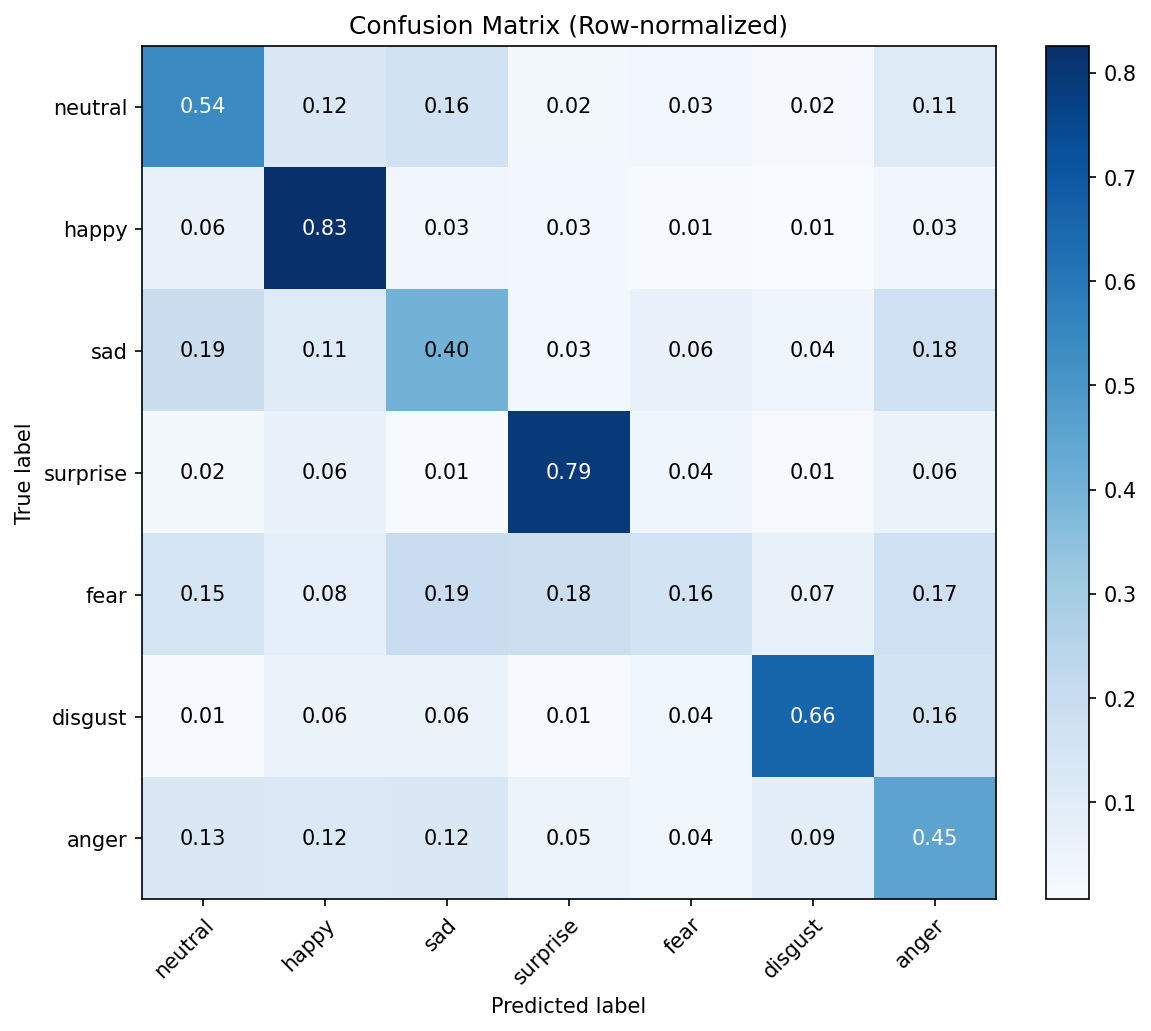
\includegraphics[width=\textwidth,height=0.70\textheight,keepaspectratio]{confusion_matrix_normalized.png}
    \end{column}
  \end{columns}
\end{frame}

\begin{frame}{Qualitative correct case: happy $\rightarrow$ happy}
  % Oral: describe that the model focuses on the mouth/smile and expressive facial regions.
  \begin{center}
    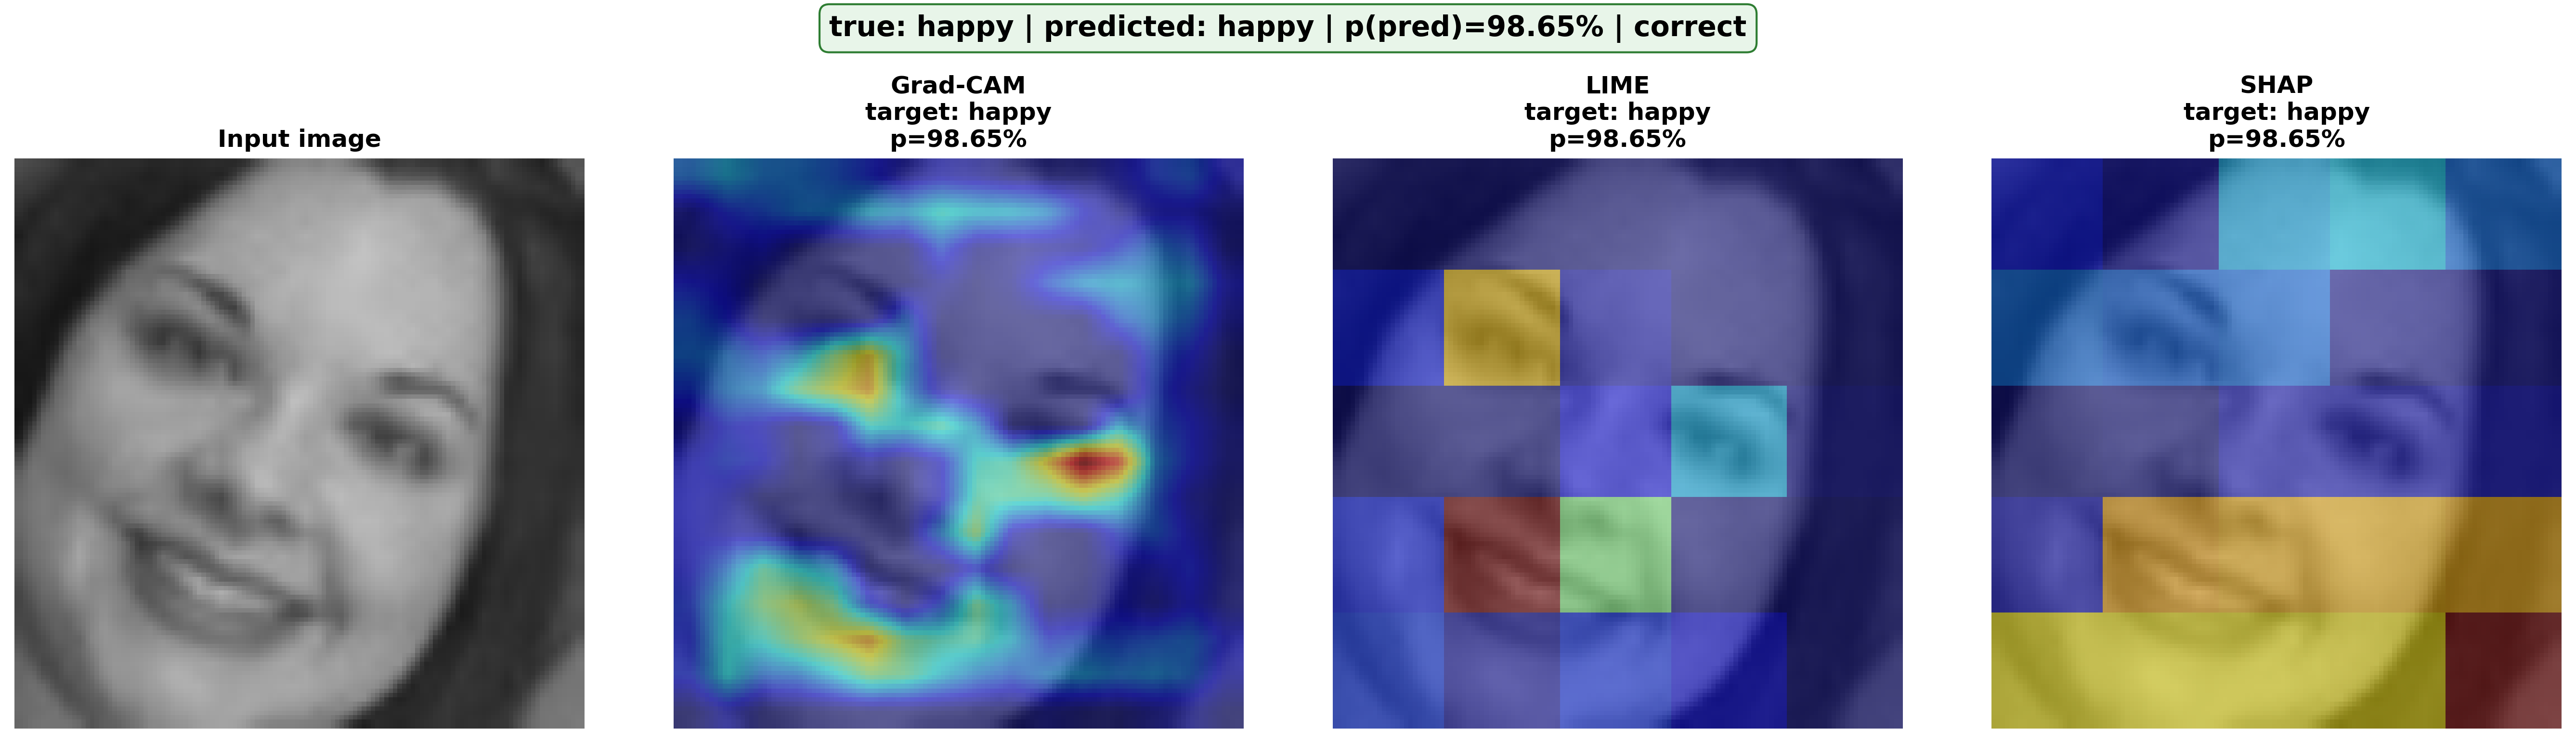
\includegraphics[width=\textwidth,height=0.78\textheight,keepaspectratio]{example_correct_happy_happy.png}
  \end{center}
  \vspace{-0.5em}
  \begin{block}{Interpretation}
    The three methods explain the class \textbf{happy}. Grad-CAM is smoother, while LIME and SHAP highlight more discrete regions. The focus on the mouth and expressive facial traits is plausible for this prediction.
  \end{block}
\end{frame}

\begin{frame}{Qualitative failure case: anger $\rightarrow$ happy}
  % Oral: this is a key slide. The error becomes interpretable: apparent smile, mouth/eye regions.
  \begin{center}
    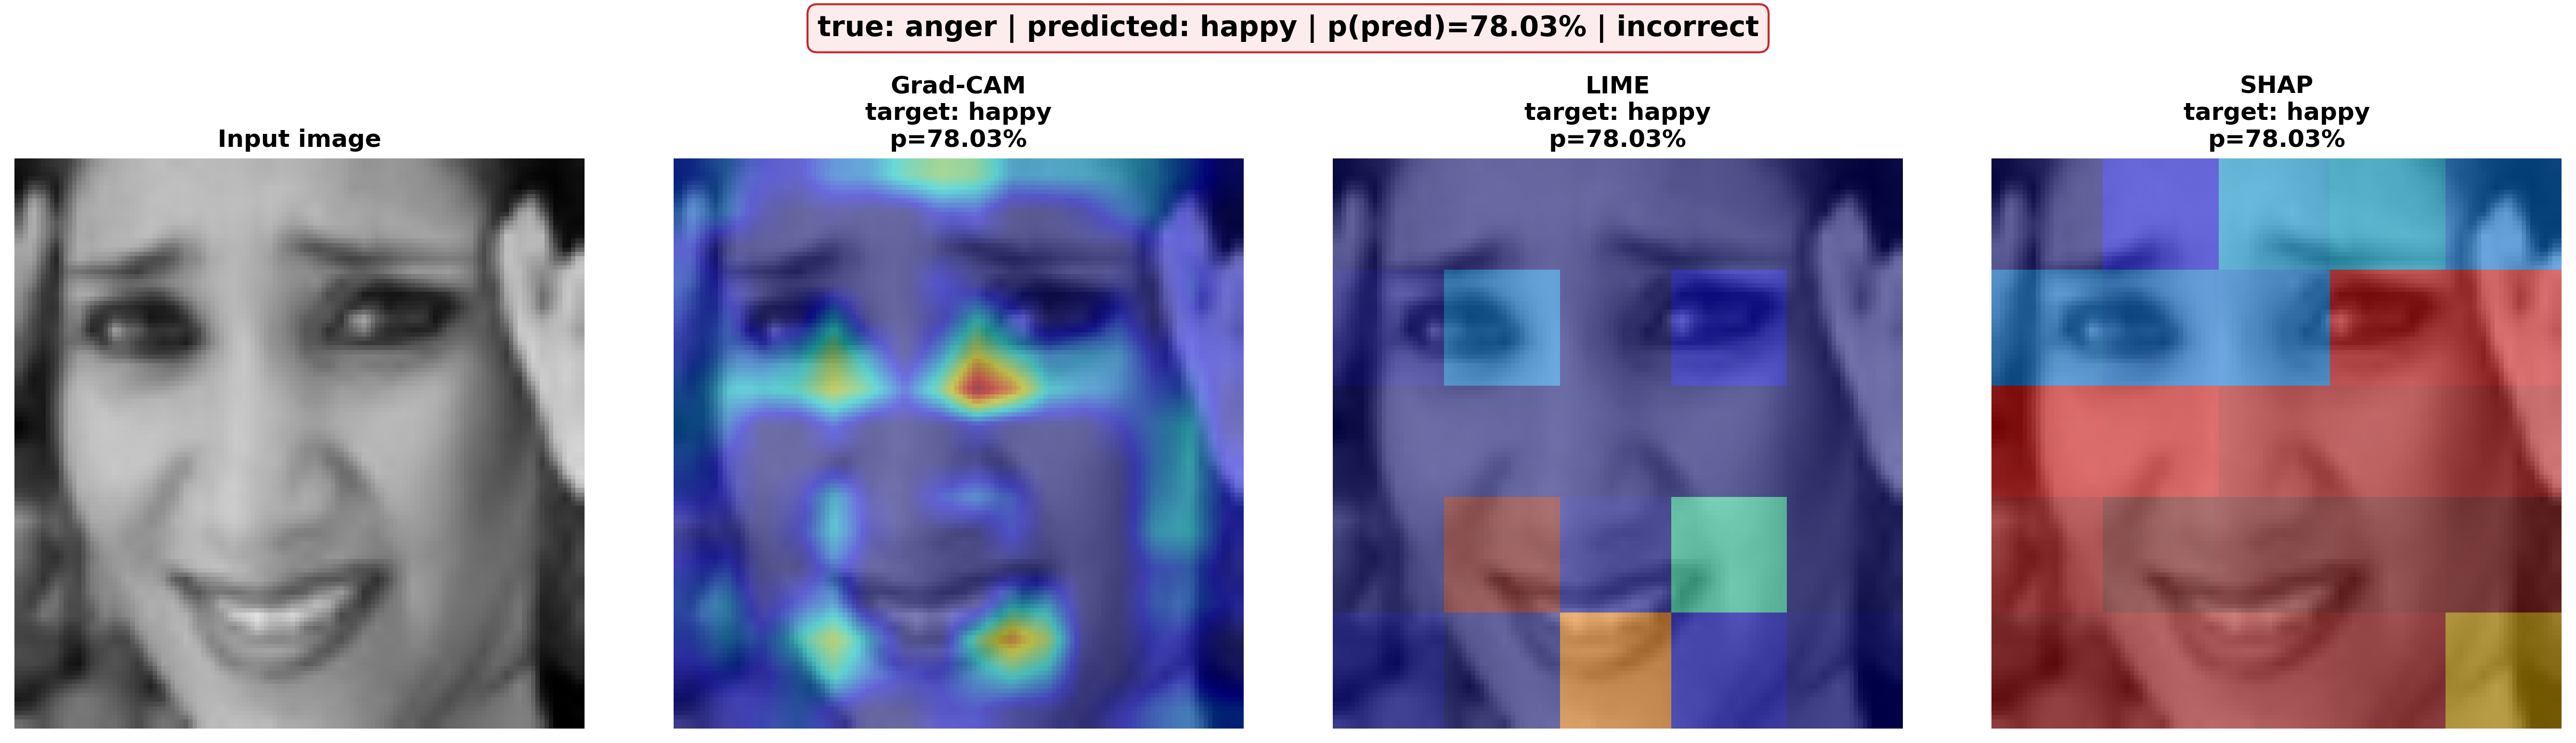
\includegraphics[width=\textwidth,height=0.78\textheight,keepaspectratio]{example_incorrect_anger_happy.png}
  \end{center}
  \vspace{-0.5em}
  \begin{alertblock}{Why this image matters}
    The true label is \textbf{anger}, but the model predicts \textbf{happy}. The explanations show that the model relies on regions compatible with a smile; the error is not random, it reveals a semantic confusion.
  \end{alertblock}
\end{frame}

\begin{frame}{Quantitative comparison of XAI methods}
  % Oral: emphasize the trade-off: LIME is most faithful, Grad-CAM more stable, SHAP less reliable in this setup.
  \begin{center}
    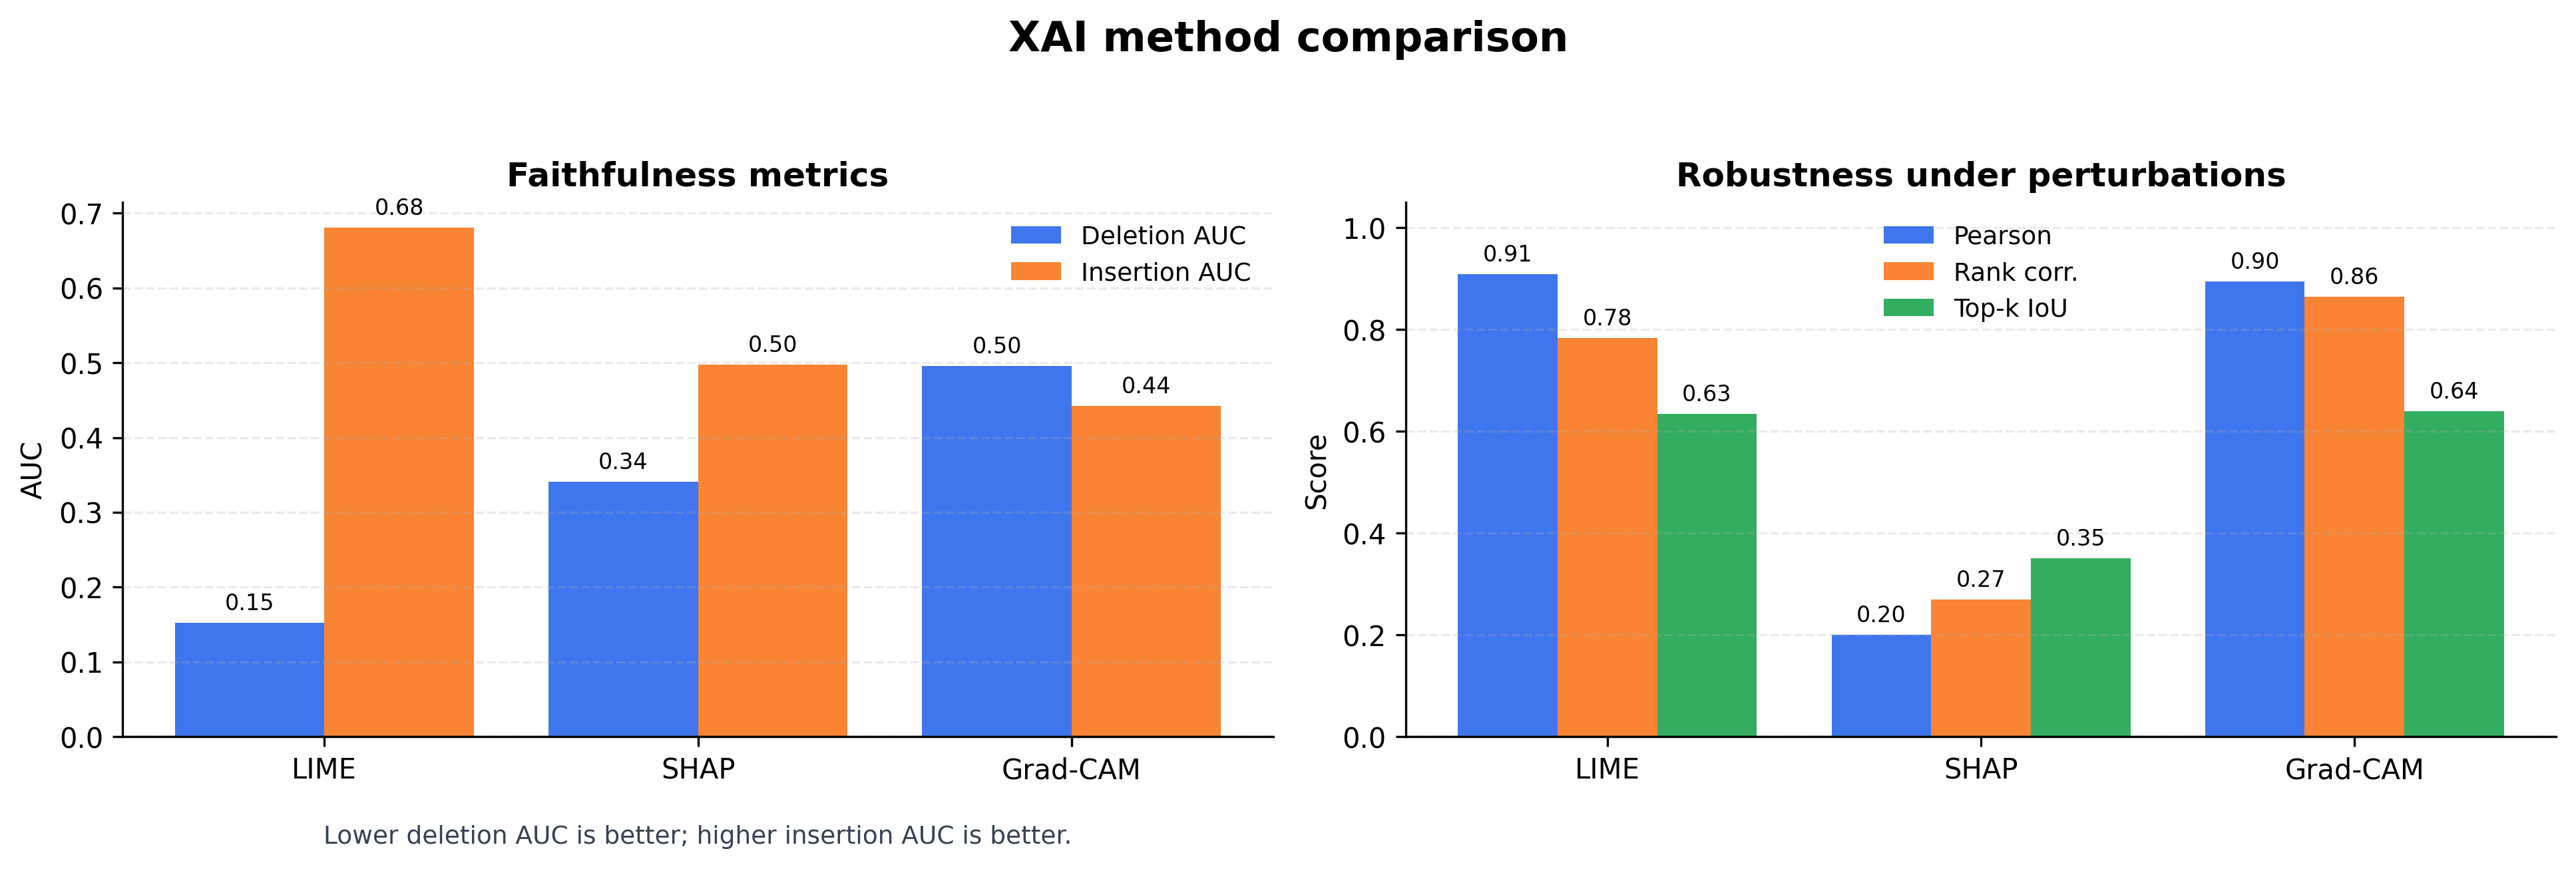
\includegraphics[width=\textwidth,height=0.56\textheight,keepaspectratio]{xai_method_summary.png}
  \end{center}
  \vspace{-0.3em}
  \small
  \begin{columns}[T,totalwidth=\textwidth]
    \begin{column}{0.49\textwidth}
      \begin{block}{Faithfulness}
        LIME has the best combination: lower deletion AUC and higher insertion AUC.
      \end{block}
    \end{column}
    \begin{column}{0.49\textwidth}
      \begin{block}{Robustness}
        Grad-CAM and LIME remain stable; SHAP is more sensitive to perturbations in our approximation.
      \end{block}
    \end{column}
  \end{columns}
\end{frame}

\begin{frame}{Facial-region masking analysis}
  % Oral: connect to FER domain knowledge. The mouth has the strongest causal effect on predictions.
  \begin{center}
    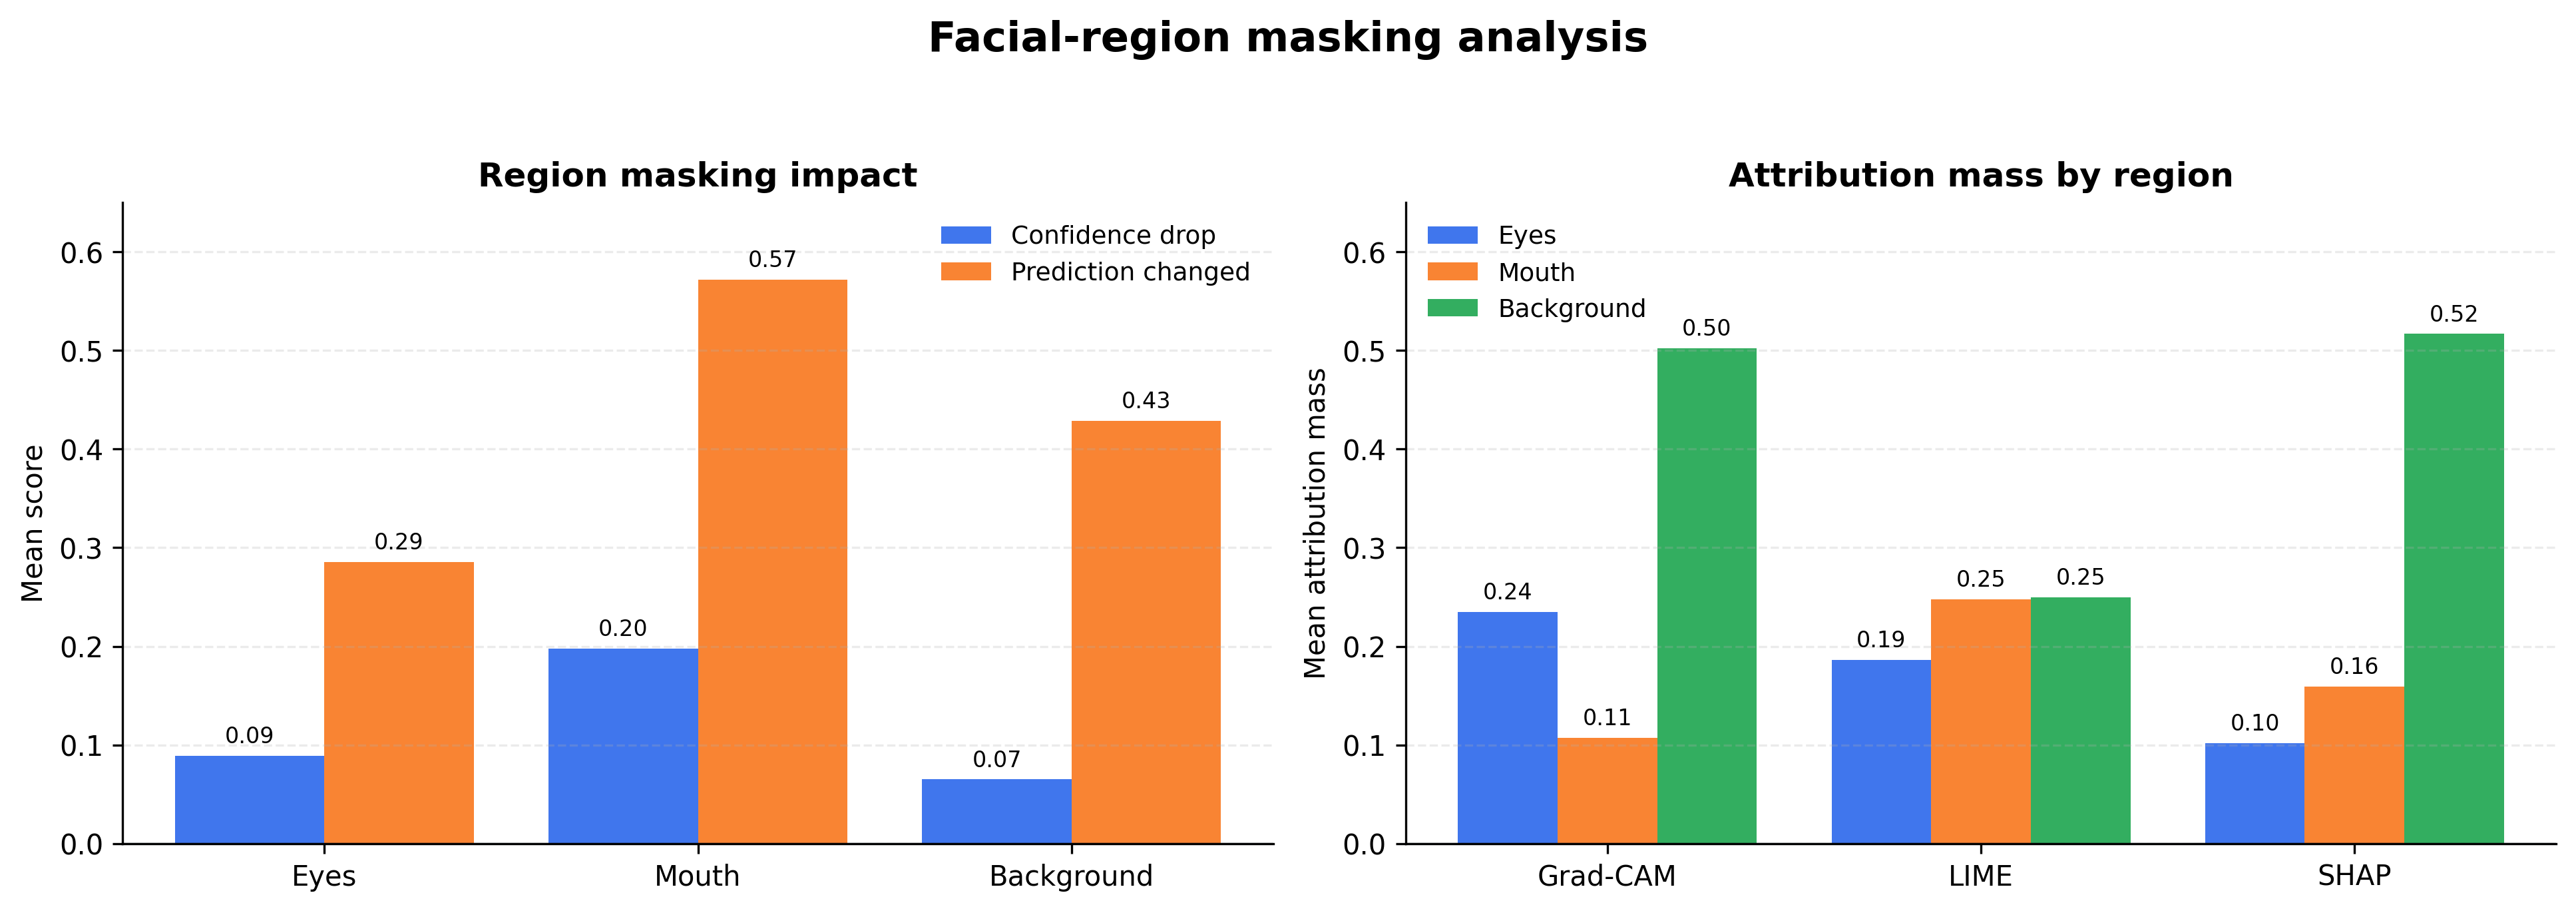
\includegraphics[width=\textwidth,height=0.56\textheight,keepaspectratio]{masking_summary.png}
  \end{center}
  \vspace{-0.3em}
  \small
  \begin{block}{Main result}
    Masking the \textbf{mouth} causes the largest average confidence drop and changes the prediction in 57\% of analyzed cases. This is consistent with facial expression recognition, but it also shows that the model may over-rely on specific local cues.
  \end{block}
\end{frame}

\begin{frame}{Discussion: what do we actually learn?}
  % Oral: be balanced and evidence-based. Do not overclaim.
  \begin{columns}[T,totalwidth=\textwidth]
    \begin{column}{0.49\textwidth}
      \begin{block}{Strengths}
        \begin{itemize}
          \item End-to-end pipeline: training, evaluation, XAI.
          \item Comparison of three families of methods.
          \item Visual and quantitative evaluation.
          \item Error analysis, not only successful cases.
        \end{itemize}
      \end{block}
      \begin{block}{Messages}
        \begin{itemize}
          \item LIME is most faithful on the analyzed sample.
          \item Grad-CAM is stable and readable.
          \item SHAP is less robust here with the grid approximation.
        \end{itemize}
      \end{block}
    \end{column}
    \begin{column}{0.49\textwidth}
      \begin{alertblock}{Limitations}
        \begin{itemize}
          \item Full XAI analysis computed on 7 images due to cost.
          \item LIME/SHAP regions are coarse because they rely on a grid.
          \item The FER model is not optimized for state-of-the-art accuracy.
          \item Eye/mouth/background masks remain approximate.
        \end{itemize}
      \end{alertblock}
    \end{column}
  \end{columns}
\end{frame}

\begin{frame}{Conclusion and take-home messages}
  % Oral: end clearly. The teacher should leave with three ideas.
  \begin{block}{Answer to the research question}
    XAI methods are not interchangeable: on our FER model, they produce visually and quantitatively different explanations.
  \end{block}

  \begin{columns}[T,totalwidth=\textwidth]
    \begin{column}{0.32\textwidth}
      \begin{block}{1. Fidelity}
        LIME is the most convincing method in deletion/insertion tests on our sample.
      \end{block}
    \end{column}
    \begin{column}{0.32\textwidth}
      \begin{block}{2. Stability}
        Grad-CAM is more stable and easier to interpret, but less faithful quantitatively.
      \end{block}
    \end{column}
    \begin{column}{0.32\textwidth}
      \begin{block}{3. Failure analysis}
        Model errors become interpretable: some confusions arise from ambiguous facial cues.
      \end{block}
    \end{column}
  \end{columns}

  \vspace{0.8em}
  \begin{alertblock}{Future work}
    Extend the XAI analysis to more images, use more anatomical superpixels, and train a variant with explanation-guided regularization.
  \end{alertblock}
\end{frame}

\appendix

\begin{frame}{Backup: per-class details}
  \small
  \begin{table}
    \begin{tabular}{l r r r r}
      \toprule
      Class & Precision & Recall & F1 & Support \\
      \midrule
      neutral & 0.512 & 0.541 & 0.526 & 930 \\
      happy & 0.733 & 0.826 & 0.777 & 1349 \\
      sad & 0.447 & 0.399 & 0.422 & 912 \\
      surprise & 0.646 & 0.792 & 0.712 & 600 \\
      fear & 0.438 & 0.158 & 0.232 & 768 \\
      disgust & 0.230 & 0.659 & 0.341 & 82 \\
      anger & 0.409 & 0.452 & 0.430 & 743 \\
      \bottomrule
    \end{tabular}
  \end{table}
  \begin{block}{How to use this slide}
    If asked why the global score is not higher: RAF-DB is imbalanced and some emotions are naturally confused, especially fear, sad, surprise and anger.
  \end{block}
\end{frame}

\begin{frame}{Backup: files and reproducibility}
  \begin{block}{Main commands}
    \small
    \texttt{py -3 -m src.main\_evaluate\_all --config configs/main\_cnn\_v1.yaml --checkpoint experiments/checkpoints/best\_model150epochs.pt}\\[0.4em]
    \texttt{py -3 -m src.main\_compare\_xai --config configs/main\_cnn\_xai.yaml --checkpoint experiments/checkpoints/best\_model150epochs.pt --output\_dir experiments/xai\_clean}
  \end{block}
  \begin{block}{Figures used}
    \small
    \pathfig{experiments/xai_clean/report_figures/}
  \end{block}
  \begin{block}{Quantitative outputs}
    \small
    \pathfig{xai_method_summary.csv}, \pathfig{xai_masking_summary.csv}, \pathfig{test_overall_metrics.csv}
  \end{block}
\end{frame}

\begin{frame}{Backup: peer-reviewed references}
  \scriptsize
  \begin{thebibliography}{99}
    \bibitem{rafdb} S. Li, W. Deng, and J. Du. Reliable Crowdsourcing and Deep Locality-Preserving Learning for Expression Recognition in the Wild. CVPR, 2017.
    \bibitem{gradcam} R. R. Selvaraju et al. Grad-CAM: Visual Explanations from Deep Networks via Gradient-Based Localization. ICCV, 2017.
    \bibitem{lime} M. T. Ribeiro, S. Singh, and C. Guestrin. Why Should I Trust You? Explaining the Predictions of Any Classifier. KDD, 2016.
    \bibitem{shap} S. M. Lundberg and S.-I. Lee. A Unified Approach to Interpreting Model Predictions. NeurIPS, 2017.
    \bibitem{sanity} J. Adebayo et al. Sanity Checks for Saliency Maps. NeurIPS, 2018.
    \bibitem{infidelity} C.-K. Yeh et al. On the (In)fidelity and Sensitivity of Explanations. NeurIPS, 2019.
  \end{thebibliography}
  \vspace{0.7em}
  \begin{block}{Credibility check}
    These references are standard XAI / FER papers from CVPR, ICCV, KDD and NeurIPS, and directly justify the dataset, methods and evaluation protocol.
  \end{block}
\end{frame}

\end{document}
